\begin{landscape}
\begin{singlespacing}
\begin{small}
\begin{longtable}{>{\textsf\bgroup}p{3.5cm}<{\egroup} >{\textsf\bgroup}p{4cm}<{\egroup} >{\textsf\bgroup}p{8cm}<{\egroup}>{\textsf\bgroup}p{6.5cm}<{\egroup}} % defining the columns - these must match the widths defined for the mini pages down below!
\caption[Peak calling strategies adjusted for the different sample characteristics.]{\textsf{Peak calling strategies adjusted for the different ChIP-seq sample characteristics.}} \\ % the \\ is important! 
%%%%%%%%%%%%%%%
% table title
\textbf{ChIP-seq sample} & \textbf{Issues} & \textbf{Strategy} &  % 
\tabularnewline \hline
\endfirsthead % indicates that the lines above appear as head of the table on the first page
\multicolumn{4}{c} 
{\tablename\ \thetable\ -- \textit{Continued from previous page}} \\
\textbf{ChIP-seq samples} & \textbf{Issues} & \textbf{Strategy} &  % 
\tabularnewline \toprule \tabularnewline [1ex]
\endhead % Line(s) to appear at top of every page (except first)
\hline \multicolumn{4}{r}{\textit{Continued on next page}} \\ %
\endfoot % Last line(s) to appear at the bottom of every page (except last)
\endlastfoot
%%%%%%%%%%%%%%%%%%%
%%% let's start the table content; each column (often) gets its own minipage which enables itemized lists etc.
%%%%%%%%%%%%%%%%%%%
%% first row
%-----------------------
\toprule
\begin{minipage}[c]{3.5cm}
NSL1, NSL3,\\MCRS2, MBD-R2 in\\\textit{D.~melanogaster}
\end{minipage}
			& \begin{minipage}[c]{4cm}
			peak regions often contained more than one local maximum due to the gene-dense nature of the \textit{Drosophila} genome
			\end{minipage}
				& \begin{minipage}[c]{8cm}
				\begin{enumerate}[noitemsep, leftmargin=*]
					\item peak calling with MACS 1.4.2 with default parameters \citep{Feng2012}
					\item peaks with FDR $\leq$ 5\%
					\item identification of smaller \textsl{subpeaks} with PeakSplitter \citep{Salmon2010}
				\end{enumerate}
				\end{minipage}
					& \begin{minipage}[c]{6.5cm}
					\parbox[c]{1em}{
						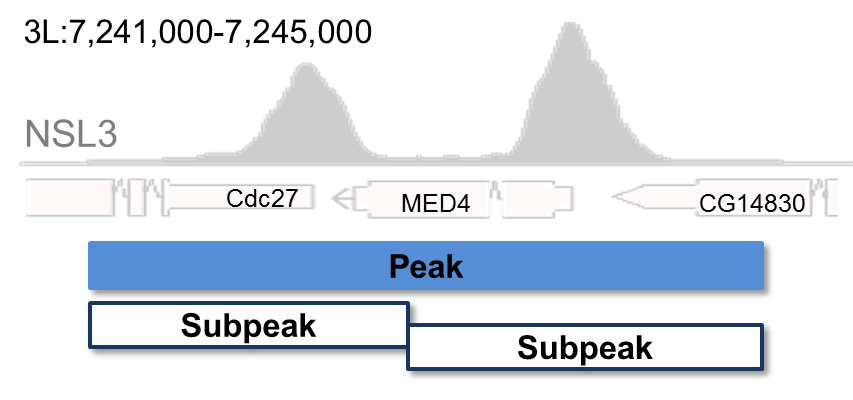
\includegraphics[width=6.5cm,trim=2 2 2 2,clip]{Figures/PeakCalling_Dmel}}
				\end{minipage} 
%\\ [2ex]  \hline \\ [1ex]
\tabularnewline \midrule
%-----------------------
\begin{minipage}[c]{3.5cm}
Pol~II in\\\textit{D.~melanogaster} cells\\(depleted of NSL1 or NSL3)
\end{minipage}
	& \begin{minipage}[c]{4cm}
	the mixed signal of Pol~II (localized, TF-like enrichments around TSS, broad, shallow enrichments along gene bodies) was not well captured by MACS
		\end{minipage}
		& \begin{minipage}[c]{8cm}
\vskip 6pt
				\begin{enumerate}[noitemsep, leftmargin=*]
					\item a symmetric null distribution was fitted to regions with negative enrichments, i.e. where the input signal exceeded the ChIP signal \citep{EBIroutine} (black line)
					\item genomic bins that deviated from the expectation (compare the blue with the black line) were determined as significantly enriched (threshold: q-value $\leq$ 0.05) \\ [2ex]
				\end{enumerate}
\vskip 4pt
			\end{minipage}
				& \begin{minipage}[c]{6.5cm}
						\parbox[c]{1em}{
						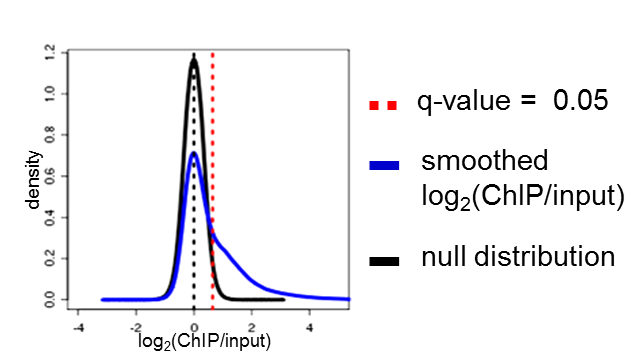
\includegraphics[width=6.5cm,trim=4 4 4 4,clip]{Figures/PeakCalling_PolII}}
					\end{minipage}
%\\ [2ex] \hline \\ [1ex]
\tabularnewline \midrule
%-----------------------
\begin{minipage}[c]{3.5cm}
MOF, MSL1, MSL2,\\NSL3, MCRS1 in\\ mouse ESCs and NPCs
\end{minipage}
	& \begin{minipage}[c]{4cm}
	non-optimal signal-noise ratios, GC bias
		\end{minipage}
		& \begin{minipage}[c]{8cm}
\vskip 6pt
				\begin{enumerate}[noitemsep, leftmargin=*]
                    \item in ESCs: adjustment of the GC bias in the input sample to match each ChIP-seq sample's GC bias
					\item peak calling with MACS 1.4.2 with default parameters \citep{Feng2012} for each ChIP-seq replicate (blue boxes) and the merged file (red box)
					\item only peaks that were present in both replicates and met the FDR threshold of $\leq$ 1\% were used \\ [2ex]
				\end{enumerate}
\vskip 4pt
			\end{minipage}
				& \begin{minipage}[c]{6.5cm}
\vskip 6pt
						\parbox[c]{1em}{
						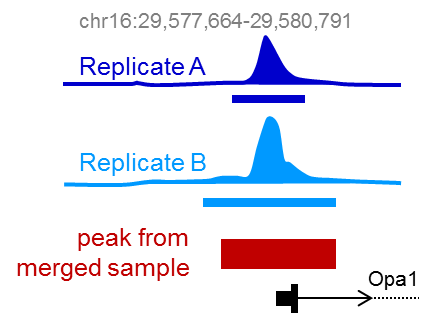
\includegraphics[width=5.5cm,trim=4 4 4 4,clip]{Figures/PeakCalling_Mm}} 
\vskip 4pt
					\end{minipage}
%\\ [2ex] \hline \\ [1ex]
%-----------------------
\tabularnewline \bottomrule
\label{tab:peakCallingStrategies}
\end{longtable}
\end{small}
\end{singlespacing}
\end{landscape}
